This appendix contains details on the experiments measuring human ability to distinguish GPT-3-generated synthetic news articles from real news articles. We first describe the experiments on the $\sim200$ word news articles, and then describe the preliminary investigation of $\sim500$ word news articles generated by GPT-3.

\textit{Participants:} We recruited 718 unique participants to take part in 6 experiments. 97 participants were excluded  for failing an internet check question, leaving a total of 621 participants: 343 male, 271 female, and 7 other. Mean participant age was $\sim38$ years old. All participants were recruited through Positly, which maintains a whitelist of high-performing workers from Mechanical Turk. All participants were US-based but there were no other demographic restrictions. Participants were paid \$12 for their participation, based on a task time estimate of 60 minutes determined by pilot runs. In order to ensure that the sample of participants for each experiment quiz was unique, participants were not allowed to take part in an experiment more than once.

\textit{Procedure and design:} We arbitrarily selected 25 news articles that appeared in \href{newser.com}{newser.com} in early 2020. We used the article titles and subtitles to produce outputs from the 125M, 350M, 760M, 1.3B, 2.7B, 6.7B, 13.0B, and 200B (GPT-3) parameter language models. Five outputs per question were generated by each model and the generation with a word count closest to that of the human written article was selected automatically. This was to minimize the effect that completion length might have on participants’ judgments.  The same output procedure for each model with the exception of the removal of the intentionally bad control model, as described in the main text. 

In each experiment, half of the participants were randomly assigned to quiz A and half were randomly assigned to quiz B. Each quiz consisted of 25 articles: half (12-13) were human written and half (12-13) were model generated: the articles with human written completions in quiz A had model generated completions in quiz B and vice versa. The order of quiz question was shuffled for each participant. Participants could leave comments and were asked to indicate if they had seen the articles before. Participants were instructed not to look up the articles or their content during the quiz and at the end of the quiz were asked if they had looked anything up during the quiz.

\begin{table}
    \begin{center}
        \begin{tabular}{l c c c c c}
        \toprule
        Model & \shortstack{Participants\\Recruited}  & \shortstack{Participants\\Excluded} & \shortstack{Genders\\(m:f:other)} & \shortstack{Mean\\Age} & \shortstack{Average\\Word Count\\(human:model)} \\ 
        \midrule
        Control  & 76 & 7 & 32:37:0 & 39 & 216:216 \\ 
        GPT-3 Small  & 80 & 7  & 41:31:1 & 40 & 216:188 \\ 
        GPT-3 Medium  & 80 & 7  & 46:28:2  & 39 & 216:202 \\ 
        GPT-3 Large  & 81 & 24  & 46:28:2  & 37 & 216:200 \\ 
        GPT-3 XL  & 79 & 14  & 32:32:1  & 38 & 216:199 \\ 
        GPT-3 2.7B  & 80 & 11  & 36:33:0  & 40 & 216:202 \\ 
        GPT-3 6.7B  & 76 & 5  & 46:28:2  & 37 & 216:195 \\ 
        GPT-3 13.0B  & 81 & 13  & 46:28:2  & 37 & 216:209 \\ 
        GPT-3 175B & 80 & 9  & 42:29:0 &  37 & 216:216 \\ 
        \bottomrule
        \end{tabular}
    \end{center}
    \caption{Participant details and  article lengths for each experiment to evaluate human detection of $\sim200$ word model generated news articles. Participants were excluded due to internet check fails.}
    \label{table:study}
\end{table}

\textit{Statistical Tests:} To compare means on the different runs, we performed a two-sample t-test for independent groups for each model against the control. This was implemented in Python using the \verb|scipy.stats.ttest_ind| function. When plotting a regression line in the graph of average participant accuracy vs model size, we fit a power law of the form $ax^{-b}$. The 95\% confidence intervals were estimated from the t-distribution of the sample mean.

\begin{figure}
\centering
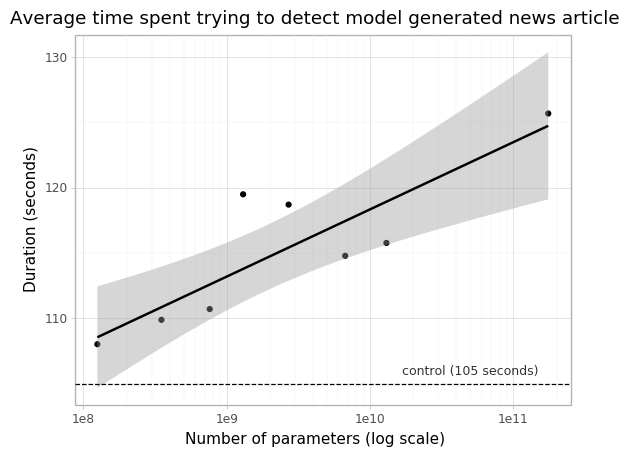
\includegraphics[width=0.7\linewidth]{graphs/img/newsduration.png}
\caption{Participants spend more time trying to identify whether each news article is machine generated as model size increases.  Duration on the control model is indicated with the dashed line. Line of best fit is a linear model on a log scale with 95\% confidence intervals.}
\label{graph:newsduration}
\end{figure}

\textit{Duration statistics}: In the main text, we discussed the finding that the ability of human participants to distinguish model and human generated news articles decreases as our models become larger. We have also found that the average time spent for a given set of questions increases as the model size increases, as shown in Figure \ref{graph:newsduration}. Lower accuracy scores despite increased time investment from participants supports the finding that larger models generate harder-to-distinguish news articles.

\textit{Preliminary investigation of $\sim500$ word articles:} We recruited 160 unique US-based participants to take part in 2 experiments through Positly (details are given in Table \ref{table:study_long}). We randomly selected 12 Reuters world news articles from late 2019 and created a context for GPT-3 175B that consisted of a single Reuters article not in this set of 12. We then used the article titles and Reuters locations to generate completions from GPT-3 175B and the 160M control model from the previous experiments. These were used to create two 12-question quizzes per model, each consisting of half human written and half model generated articles. Comprehension questions were added and articles were shown to participants in 3 stages at 30 second intervals to encourage closer reading. Participants were paid \$12 for this task. Model generation selection methods, exclusion criteria, and statistical tests mirror those of the previous experiments.

\begin{table}
    \begin{center}
        \begin{tabular}{l c c c c c}
        \toprule
        Model & \shortstack{Participants\\Recruited}  & \shortstack{Participants\\Excluded} & \shortstack{Genders\\(m:f:other)} & \shortstack{Mean\\Age} & \shortstack{Average\\Word Count\\(human:model)} \\ 
        \midrule
        Control  & 79 & 17 & 32:37:0 & 39 & 569:464 \\ 
        GPT-3 175B & 81 & 19  & 32:30:0 &  40 & 569:498 \\ 
        \bottomrule
        \end{tabular}
    \end{center}
    \caption{Participant details and  article lengths for the experiments investigating  human detection of $\sim500$ word model generated news articles. Participants were excluded due to internet check fails.}
    \label{table:study_long}
\end{table}